% Options for packages loaded elsewhere
\PassOptionsToPackage{unicode}{hyperref}
\PassOptionsToPackage{hyphens}{url}
%
\documentclass[
]{article}
\usepackage{lmodern}
\usepackage{amssymb,amsmath}
\usepackage{ifxetex,ifluatex}
\ifnum 0\ifxetex 1\fi\ifluatex 1\fi=0 % if pdftex
  \usepackage[T1]{fontenc}
  \usepackage[utf8]{inputenc}
  \usepackage{textcomp} % provide euro and other symbols
\else % if luatex or xetex
  \usepackage{unicode-math}
  \defaultfontfeatures{Scale=MatchLowercase}
  \defaultfontfeatures[\rmfamily]{Ligatures=TeX,Scale=1}
\fi
% Use upquote if available, for straight quotes in verbatim environments
\IfFileExists{upquote.sty}{\usepackage{upquote}}{}
\IfFileExists{microtype.sty}{% use microtype if available
  \usepackage[]{microtype}
  \UseMicrotypeSet[protrusion]{basicmath} % disable protrusion for tt fonts
}{}
\makeatletter
\@ifundefined{KOMAClassName}{% if non-KOMA class
  \IfFileExists{parskip.sty}{%
    \usepackage{parskip}
  }{% else
    \setlength{\parindent}{0pt}
    \setlength{\parskip}{6pt plus 2pt minus 1pt}}
}{% if KOMA class
  \KOMAoptions{parskip=half}}
\makeatother
\usepackage{xcolor}
\IfFileExists{xurl.sty}{\usepackage{xurl}}{} % add URL line breaks if available
\IfFileExists{bookmark.sty}{\usepackage{bookmark}}{\usepackage{hyperref}}
\hypersetup{
  hidelinks,
  pdfcreator={LaTeX via pandoc}}
\urlstyle{same} % disable monospaced font for URLs
\usepackage[margin=1in]{geometry}
\usepackage{graphicx,grffile}
\makeatletter
\def\maxwidth{\ifdim\Gin@nat@width>\linewidth\linewidth\else\Gin@nat@width\fi}
\def\maxheight{\ifdim\Gin@nat@height>\textheight\textheight\else\Gin@nat@height\fi}
\makeatother
% Scale images if necessary, so that they will not overflow the page
% margins by default, and it is still possible to overwrite the defaults
% using explicit options in \includegraphics[width, height, ...]{}
\setkeys{Gin}{width=\maxwidth,height=\maxheight,keepaspectratio}
% Set default figure placement to htbp
\makeatletter
\def\fps@figure{htbp}
\makeatother
\setlength{\emergencystretch}{3em} % prevent overfull lines
\providecommand{\tightlist}{%
  \setlength{\itemsep}{0pt}\setlength{\parskip}{0pt}}
\setcounter{secnumdepth}{-\maxdimen} % remove section numbering
\usepackage{float} \usepackage{caption} \captionsetup[table]{font=footnotesize} \captionsetup[figure]{font=footnotesize} \usepackage{setspace}\onehalfspacing \usepackage{lineno}\linenumbers
\usepackage{booktabs}
\usepackage{longtable}
\usepackage{array}
\usepackage{multirow}
\usepackage{wrapfig}
\usepackage{float}
\usepackage{colortbl}
\usepackage{pdflscape}
\usepackage{tabu}
\usepackage{threeparttable}
\usepackage{threeparttablex}
\usepackage[normalem]{ulem}
\usepackage{makecell}
\usepackage{xcolor}
\usepackage[]{natbib}
\bibliographystyle{apalike}

\author{}
\date{\vspace{-2.5em}}

\begin{document}

\textbf{Title:} Global patterns of forest autotrophic carbon fluxes

\textbf{Running head:}

\textbf{Authors:}

Rebecca Banbury Morgan\textsuperscript{1,2}

Valentine Herrmann\textsuperscript{1}

Norbert Kunert\textsuperscript{1,3}

Ben Bond-Lamberty\textsuperscript{4}

Helene C. Muller-Landau\textsuperscript{3}

Kristina J. Anderson-Teixeira\textsuperscript{1,3}*

\textbf{Author Affiliations:}

\begin{enumerate}
\def\labelenumi{\arabic{enumi}.}
\item
  Conservation Ecology Center; Smithsonian Conservation Biology
  Institute; Front Royal, VA, USA
\item
  \emph{Becky- current}
\item
  Center for Tropical Forest Science-Forest Global Earth Observatory;
  Smithsonian Tropical Research Institute; Panama, Republic of Panama
\item
  Joint Global Change Research Institute, Pacific Northwest National
  Laboratory, College Park Maryland 20740 USA
\end{enumerate}

*Corresponding Author:

phone: 1-540-635-6546

\url{fax:1-540-635-6506}

email: \href{mailto:teixeirak@si.edu}{\nolinkurl{teixeirak@si.edu}}

\textbf{Keywords:}

\textbf{Paper type:} Primary Research Article

\newpage

\#\#\#Abstract Carbon (C) fixation, allocation, and metabolism by trees
set the basis for energy and material flows in forest ecosystems and
define their interactions with Earth's changing climate. However, we
lack a cohesive synthesis on how forest carbon fluxes vary globally with
respect to climate and one another. Here, we draw upon 1319 records from
the Global Forest Carbon Database (ForC), representing all major forest
types and the nine most significant autotrophic carbon fluxes, to
comprehensively explore how C cycling in mature, undisturbed forests
varies with latitude and climate on a global scale. We show that, across
all flux variables analyzed, C cycling decreases continuously with
absolute latitude -- a finding that confirms multiple previous studies
but contradicts the idea that net primary productivity (\(NPP\)) of
temperate forests rivals that of tropical forests. C flux variables
generally displayed similar trends across latitude and multiple climate
variables, with no differences in allocation detected at this global
scale. Temperature variables in general, and mean annual temperature
(\(MAT\)) and temperature seasonality in particular, were the best
univariate predictors of C flux, explaining 19 - 71\% of variation in
the C fluxes analyzed. The effects of temperature were modified by
moisture availability, with C flux reduced under hot and dry conditions
and sometimes under very high precipitation. C fluxes increased with
growing season length, but this was never the best univariate predictor.
Within the growing season, the influence of climate on C cycling was
small but significant for a number of flux variables. These findings
clarify how forest C flux varies with latitude and climate on a global
scale. In a period of accelerating climatic change, this improved
understanding of the fundamental climatic controls on forest C cycling
sets a foundation for understanding patterns of change.

\newpage

\hypertarget{introduction}{%
\subsubsection{Introduction}\label{introduction}}

Carbon (C) cycling in Earth's forests provides the energetic basis for
sustaining the majority of Earth's terrestrial biodiversity and many
human populations
\citep{millennium_ecosystem_assessment_ecosystems_2005}, while strongly
influencing atmospheric carbon dioxide (CO\textsubscript{2}) and climate
\citep{bonan_forests_2008}. Forests' autotrophic carbon fluxes--that is,
carbon fixation, allocation, and metabolism by trees and other primary
producers--sets the energy ultimately available to heterotrophic
organisms (including microbes), in turn influencing their abundance
\citep{zak_plant_1994, niedzialkowska_species_2010} and possibly
diversity \citep{waide_relationship_1999, chu_direct_2018}. They are
linked to cycling of energy, water, and nutrients, and, critically,
influence all C stocks and define forest interactions with Earth's
changing climate. Each year, over 69 Gt of C cycle through Earth's
forests \citep{badgley_terrestrial_2019}-- a flux more than seven times
greater that of recent anthropogenic fossil fuel emissions \citep[9.5 Gt
C yr\textsuperscript{-1};][]{friedlingstein_global_2019}. As atmospheric
CO\textsubscript{2} continues to rise, driving climate change, forests
will play a critical role in shaping the future of Earth's climate
\citep{cavaleri_urgent_2015, rogelj_mitigation_2018}. However, our
understanding of the climate dependence of forest C cycling on a global
scale has been limited by analyses typically considering only one or a
few variables at a time, insufficient parsing of related variables, and
the mixing of data from forests that vary in stand age, disturbance
history, and/or management status, all of which affect C cycling
\citep{litton_carbon_2007, gillman_latitude_2015, simova_enigma_2017}.

Forest C fluxes decrease with latitude
\citep[e.g.,][]{luyssaert_co_2007, piao_forest_2010, gillman_latitude_2015, li_mapping_2019},
but studies have differed in their conclusions regarding the shape of
this relationship - quite possibly because of lack of standardization
with respect to methodology and stand history. For instance, studies
agree that gross primary productivity (\(GPP\)) increases continuously
with decreasing latitude and is indisputably highest in tropical forests
\citep{luyssaert_co_2007, beer_terrestrial_2010, jung_global_2011, badgley_terrestrial_2019, li_mapping_2019}.
In contrast, some studies have suggested that net primary productivity
(\(NPP\)), or its aboveground portion (\(ANPP\)), exhibits a less
distinct increase from temperate to tropical forests
\citep{luyssaert_co_2007}--or even a decrease \citep[but see
\citet{gillman_latitude_2015}]{huston_global_2009}. A shallower increase
in \(NPP\) than in \(GPP\) with decreasing latitude would align with the
suggestion that tropical forests tend to have low carbon use efficiency
\citep[\(CUE\)=
\(NPP\)/\(GPP\);][]{de_lucia_forest_2007, malhi_productivity_2012, anderson-teixeira_carbon_2016}.
Such differences among C fluxes their relationship to latitude could
have profound implications for our understanding of the C cycle and its
climate sensitivity. However, until recently the potential to compare
latitudinal trends across C fluxes has been limited by lack of a large
database with standardization for methodology, stand history, and
management \citep{anderson-teixeira_forc_2018}.

The latitudinal gradient in forest C flux rates, along with altitudinal
gradients \citep{girardin_net_2010, malhi_variation_2017}, is driven
primarily by climate, which is a significant driver of C fluxes across
broad spatial scales
\citep{luyssaert_co_2007, cleveland_relationships_2011, wei_forest_2010}.
However, there is little consensus as to the shapes of these
relationships or the best predictor variables. The majority of studies
have focused on exploring the relationships of C fluxes to mean annual
temperature (MAT) and mean annual precipitation (MAP), as the most
commonly reported site-level climate variables. C fluxes increase
strongly with \(MAT\) on the global scale, but whether they saturate or
potentially decrease at higher temperatures remains disputed. Some
studies have detected no deceleration or decline in \(GPP\)
\citep{luyssaert_co_2007}, \(NPP\) \citep{schuur_productivity_2003}, or
root respiration \citep[\(R_{root}\);][]{wei_forest_2010} with
increasing \(MAT\). In contrast, others have found evidence of
saturation or decline of C flux in the warmest climates;
\citet{luyssaert_co_2007} found \(NPP\) saturating at around
10\(^\circ\)C MAT; \citet{larjavaara_temperature_2012} found that
increases in \(GPP\) saturate at approximately 25\(^\circ\)C MAT, and
\citet{sullivan_long-term_2020} found that, within the tropics,
\(ANPP_{stem}\) decreases at the highest maximum temperatures. C fluxes
generally saturate at high levels of MAP, though the saturation points
identified vary from \(MAP\) of \textasciitilde1000 mm for \(R_{root}\)
\citep{wei_forest_2010} up to 2,445 mm for \(NPP\)
\citep{schuur_productivity_2003}. Interactions between MAT and MAP are
also possible; within the tropics, there is a positive interaction
between MAT and MAP in shaping \(ANPP\), such that high rainfall has a
negative effect on productivity in cooler climates, compared to a
positive effect in warmer climates \citep{taylor_temperature_2017}.
There is also evidence that C fluxes also respond to climate variables
such as temperature and precipitation seasonality
\citep{wagner_climate_2016}, cloud cover
\citep{taylor_temperature_2017}, solar radiation
\citep{beer_terrestrial_2010, fyllas_solar_2017}, and potential
evapotranspiration \citep{kerkhoff_plant_2005}; however, these are not
typically assessed in global-scale analyses of annual forest C flux.

As metrics of annual climate, MAT and MAP fail to capture variation in
climate on an intra-annual scale, including temperature and
precipitation seasonality and growing season length. Some studies have
suggested that the apparently strong relationship between MAT and C
fluxes is actually a consequence of the correlation between MAT and
growing season length
\citep{kerkhoff_plant_2005, michaletz_convergence_2014, michaletz_drivers_2018}.
Kerkhoff et al.~\citeyearpar{kerkhoff_plant_2005} and Michaletz et
al.~\citeyearpar{michaletz_convergence_2014} found no significant
relationship between growing season temperature and net primary
productivity (loosely defined to include a mix of \textbf{VARIABLES})
standardized to growing season length. While this suggests that the
influence of temperature may be limited to determining the length of the
frost-free growing season, analysis with clearly defined variables and
standardized forest ages would be necessary to test the the veracity and
generality of this hypothesis.

The recent development of the Global Forest Carbon database (ForC),
which synthesizes multiple variables and including records of stand
history
\citep{anderson-teixeira_carbon_2016, anderson-teixeira_forc_2018},
opens up the possibility for a standardized analysis of global scale
variation in multiple C fluxes and the principle climatic drivers of
these patterns. In order to approach this broad topic, we simplify the
major gaps in our knowledge to five broad questions and corresponding
hypotheses (Table 1). First, we ask how nine forest autotrophic carbon
fluxes in ForC vary with latitude. We then test how these fluxes relate
to MAT and MAP, and additionally how they respond to other, less
well-studied, climate variables. Finally, we consider the relationship
between C flux and seasonality, considering the role of seasonality in
explaining variation in carbon fluxes, and the influence of climate on C
flux standardized by growing season length.

\renewcommand{\arraystretch}{2}

\begin{landscape}\begin{table}[!h]

\caption{\label{tab:unnamed-chunk-4}Summary of research questions, corresponding hypotheses, and results. Statistically signficant support for/ rejection of hypotheses is indicated with 'yes'/'no', and '-' indicates no significant relationship. Parentheses indicate partial overall support or rejection of hypotheses across all fluxes considered.}
\centering
\resizebox{\linewidth}{!}{
\fontsize{12}{14}\selectfont
\begin{tabular}[t]{llllllllllll}
\toprule
\multicolumn{1}{c}{ } & \multicolumn{1}{c}{ } & \multicolumn{9}{c}{Forest autotrophic carbon fluxes} & \multicolumn{1}{c}{ } \\
\cmidrule(l{3pt}r{3pt}){3-11}
Questions and hypotheses (with related references) & Overall & $GPP$ & $NPP$ & $ANPP$ & $ANPP_{stem}$ & $ANPP_{foliage}$ & $BNPP$ & $BNPP_{fine.root}$ & $R_{auto}$ & $R_{root}$ & Support\\
\midrule
\addlinespace[1em]
\multicolumn{5}{l}{\textbf{Q1. How do C fluxes vary with latitude?}}\\
\hspace{1em}H1.1. C fluxes decrease continuously with latitude.\textsuperscript{1}$^{,}$\textsuperscript{2}$^{,}$\textsuperscript{3}$^{,}$\textsuperscript{10} & yes & yes & yes & yes & yes & yes & yes & yes & yes & yes & Fig. 2\\
\addlinespace[1em]
\hline
\multicolumn{5}{l}{\textbf{Q2. How do C fluxes vary with mean annual temperature (MAT) and precipitation (MAP)?}}\\
\hspace{1em}H2.1. C fluxes increase continuously with MAT.\textsuperscript{1}$^{,}$\textsuperscript{4}$^{,}$\textsuperscript{9} & yes & yes & yes & yes & yes & yes & yes & yes & yes & yes & Figs. 4, S4, S5\\
\hspace{1em}H2.2. C fluxes increase with precipitation up to at least 2000 mm yr$^{-1}$.\textsuperscript{1}$^{,}$\textsuperscript{4} & yes & yes & yes & yes & yes & yes & yes & yes & yes & yes & Figs. 4, S4, S5\\
\hspace{1em}H2.3. Temperature and precipitation jointly shape C fluxes.\textsuperscript{5} & (yes) & yes & yes & yes & yes & - & - & - & yes & - & Fig. 3, Table S3\\
\addlinespace[1em]
\hline
\multicolumn{5}{l}{\textbf{Q3. How are C fluxes related to other annual climate variables?}}\\
\hspace{1em}H3.1. C fluxes display a decelerating increase or unimodal relationship with PET. & yes & yes & yes & yes & yes & yes & yes & yes & yes & yes & Figs. 4, S4, S5\\
\hspace{1em}H3.2. C fluxes display a decelerating increase or unimodal relationship with vapour pressure deficit. & yes & yes & yes & yes & yes & yes & yes & yes & yes & yes & Figs. 4, S4, S5\\
\hspace{1em}H3.3. C fluxes increase with solar radiation. & (yes) & yes & yes & yes & yes & yes & yes & yes & yes & - & Figs. S4, S5\\
\addlinespace[1em]
\hline
\multicolumn{5}{l}{\textbf{Q4. How does seasonality influence annual C fluxes?}}\\
\hspace{1em}H4.1. C fluxes decrease with temperature seasonality. & yes & yes & yes & yes & yes & yes & yes & yes & yes & yes & Figs. 4, S6, S7\\
\hspace{1em}H4.2. C fluxes decrease with precipitation seasonality. & - & - & - & - & no & - & - & - & - & - & Figs. S6, S7\\
\hspace{1em}H4.3. C fluxes increase with growing season length.\textsuperscript{6}$^{,}$\textsuperscript{7}$^{,}$\textsuperscript{8} & yes & yes & yes & yes & yes & yes & yes & yes & yes & yes & Figs. 4, S6, S7\\
\hspace{1em}H4.4. Growing season length is a better predictor of C fluxes than MAT.\textsuperscript{7}$^{,}$\textsuperscript{8} & (no) & no & no & no & - & no & no & no & no & no & Table S4\\
\addlinespace[1em]
\hline
\multicolumn{5}{l}{\textbf{Q5. When standardised by growing season length, how do annual C fluxes vary with climate?}}\\
\hspace{1em}H5.1. Growing season C fluxes increase with temperature.\textsuperscript{8} & (yes) & - & - & yes & - & yes & - & - & - & - & Figs. S8, S9\\
\hspace{1em}H5.2. Growing season C fluxes increase with PET. & (yes) & yes & yes & - & yes & - & yes & yes & - & - & Figs. S8, S9\\
\hspace{1em}H5.3. Growing season C fluxes increase with precipitation. & (yes) & - & - & yes & - & yes & - & - & - & - & Figs. S8, S9\\
\hspace{1em}H5.4. Growing season C fluxes increase with solar radiation. & (yes) & - & - & - & - & - & yes & yes & - & - & Figs. S8, S9\\
\bottomrule
\multicolumn{12}{l}{\textsuperscript{1} Luyssaert et al. (2007) \textsuperscript{2} Gillman et al. (2015) \textsuperscript{3} Simova and Storch (2017) \textsuperscript{4} Schuur (2003) \textsuperscript{5} Taylor et al. (2016) \textsuperscript{6} Malhi (2012) \textsuperscript{7} Michaletz et al. (2014) \textsuperscript{8} Chu et al. (2016) \textsuperscript{9} Piao et al. (2010) \textsuperscript{10} Huston \& Wolverton (2009)}\\
\end{tabular}}
\end{table}
\end{landscape}

\hypertarget{materials-and-methods}{%
\subsubsection{Materials and Methods}\label{materials-and-methods}}

\emph{Forest carbon flux data}

This analysis focused on nine C flux variables included in the
open-access ForC database (Table 2)
\citep{anderson-teixeira_carbon_2016, anderson-teixeira_forc_2018}. ForC
contains records of field-based measurements of forest carbon stocks and
annual fluxes, compiled from original publications and existing data
compilations and databases. Associated data, such as stand age,
measurement methodologies, and disturbance history, are also included.
The database was significantly expanded since the publication of
\citet{anderson-teixeira_forc_2018} through integration with the Global
Soil Respiration Database \citep{bond-lamberty_global_2010}. Additional
targeted literature searches were conducted to identify further
available data on the fluxes analyzed here, with particular focus on
mature forests in temperate and boreal regions, which were not included
in the review of \citet{anderson-teixeira_carbon_2016}. We used ForC
v3.0, archived on Zenodo with DOI 10.5281/zenodo.3403855. This version
contained 29,730 records from 4,979 plots, representing 20 distinct
ecozones across all forested biogeographic and climate zones.

This analysis focused on mature forests with no known history of
signficant disturbance or management. There is evidence that stand age
influences patterns of C flux and allocation in forest ecosystems, and
can confound relationships between latitude and primary productivity
\citep{de_lucia_forest_2007, gillman_latitude_2015}. To reduce any
biasing effects of stand age, we included only stands of known age
\(\ge\) 100 years and those described by terms such as ``mature'',
``intact'', or ``old-growth''. Since management can alter observed
patterns of C cycling \citep{simova_enigma_2017}, sites were excluded
from analysis if they were managed, defined as plots that were planted,
managed as plantations, irrigated, fertilised or including the term
``managed'' in their site description. Sites that had experienced
significant disturbance within the past 100 years were also excluded.
Disturbances that qualified sites for exclusion included major cutting
or harvesting, burning, flooding, drought and storm events with site
mortality \textgreater10\% of trees. Grazed sites were retained.

\begin{table}[!h]

\caption{\label{tab:unnamed-chunk-5}Definitions and sample sizes of carbon flux variables used in analysis. All variables are in units of Mg C ha$^{-1}$ yr$^{-1}$. }
\centering
\resizebox{\linewidth}{!}{
\fontsize{12}{14}\selectfont
\begin{tabular}[t]{l>{\raggedright\arraybackslash}p{4cm}>{\raggedright\arraybackslash}p{7cm}>{\raggedright\arraybackslash}p{10cm}>{\raggedleft\arraybackslash}p{1.5cm}>{\raggedleft\arraybackslash}p{1.5cm}}
\toprule
\multicolumn{1}{c}{ } & \multicolumn{1}{c}{ } & \multicolumn{1}{c}{ } & \multicolumn{1}{c}{ } & \multicolumn{2}{c}{Sample size} \\
\cmidrule(l{3pt}r{3pt}){5-6}
Variable & Definition & Components included & Methodologies & records & geographic areas\textsuperscript{*}\\
\midrule
$GPP$ & Gross Primary Production & full ecosystem & flux partitioning of eddy-covariance; $NPP$+$R_{auto}$ & 243 & 49\\
$NPP$ & Net Primary Production & stem, foliage, coarse root, fine root, optionally others (e.g., branch, reproductive, understory) & $ANPP$ + $BNPP$ (majority); $GPP$-$R_{auto}$ & 161 & 56\\
$ANPP$ & Aboveground $NPP$ & stem, foliage, optionally others (e.g., branch, reproductive, understory) & $ANPP_{stem}$ + $ANPP_{foliage}$ (+ others) & 278 & 86\\
$ANPP_{stem}$ & Stem growth component of $ANPP$ & woody stems down to DBH $\le$ 10cm (no branch turnover) & stem growth measurements scaled to biomass using allometries & 264 & 96\\
$ANPP_{foliage}$ & Foliage component of $ANPP$ & foliage & litterfall collection, with separation into components & 98 & 49\\
\addlinespace
$BNPP$ & Belowground $NPP$ & coarse and fine roots & coarse roots estimated indirectly using allometries based on aboveground stem increment measures ; fine roots as below & 101 & 48\\
$BNPP_{fine.root}$ & Fine root component of $BNPP$ & fine roots & measurements combined one or more of the following: soil cores, minirhizotrons, turnover estimates,  root ingrowth cores & 88 & 41\\
$R_{auto}$ & Autotrophic respiration & foliage, stem, and root & chamber measurements of foliage and stem gas exchange +  $R_{root}$ (as below) & 22 & 13\\
$R_{root}$ & Root respiration & (coarse and) fine roots & partitioning of total soil respiration (e.g., through root exclusion), scaling of root gas exchange; excluded alkali absoption and soda lime methods for measuring soil respiration & 64 & 26\\
\bottomrule
\multicolumn{6}{l}{\textsuperscript{*} Geographic areas group geographically proximate sites, defined using a hierarchical cluster analysis on the distance matrix of the sites, and a cutoff of 25km}\\
\end{tabular}}
\end{table}

\begin{figure}[H]
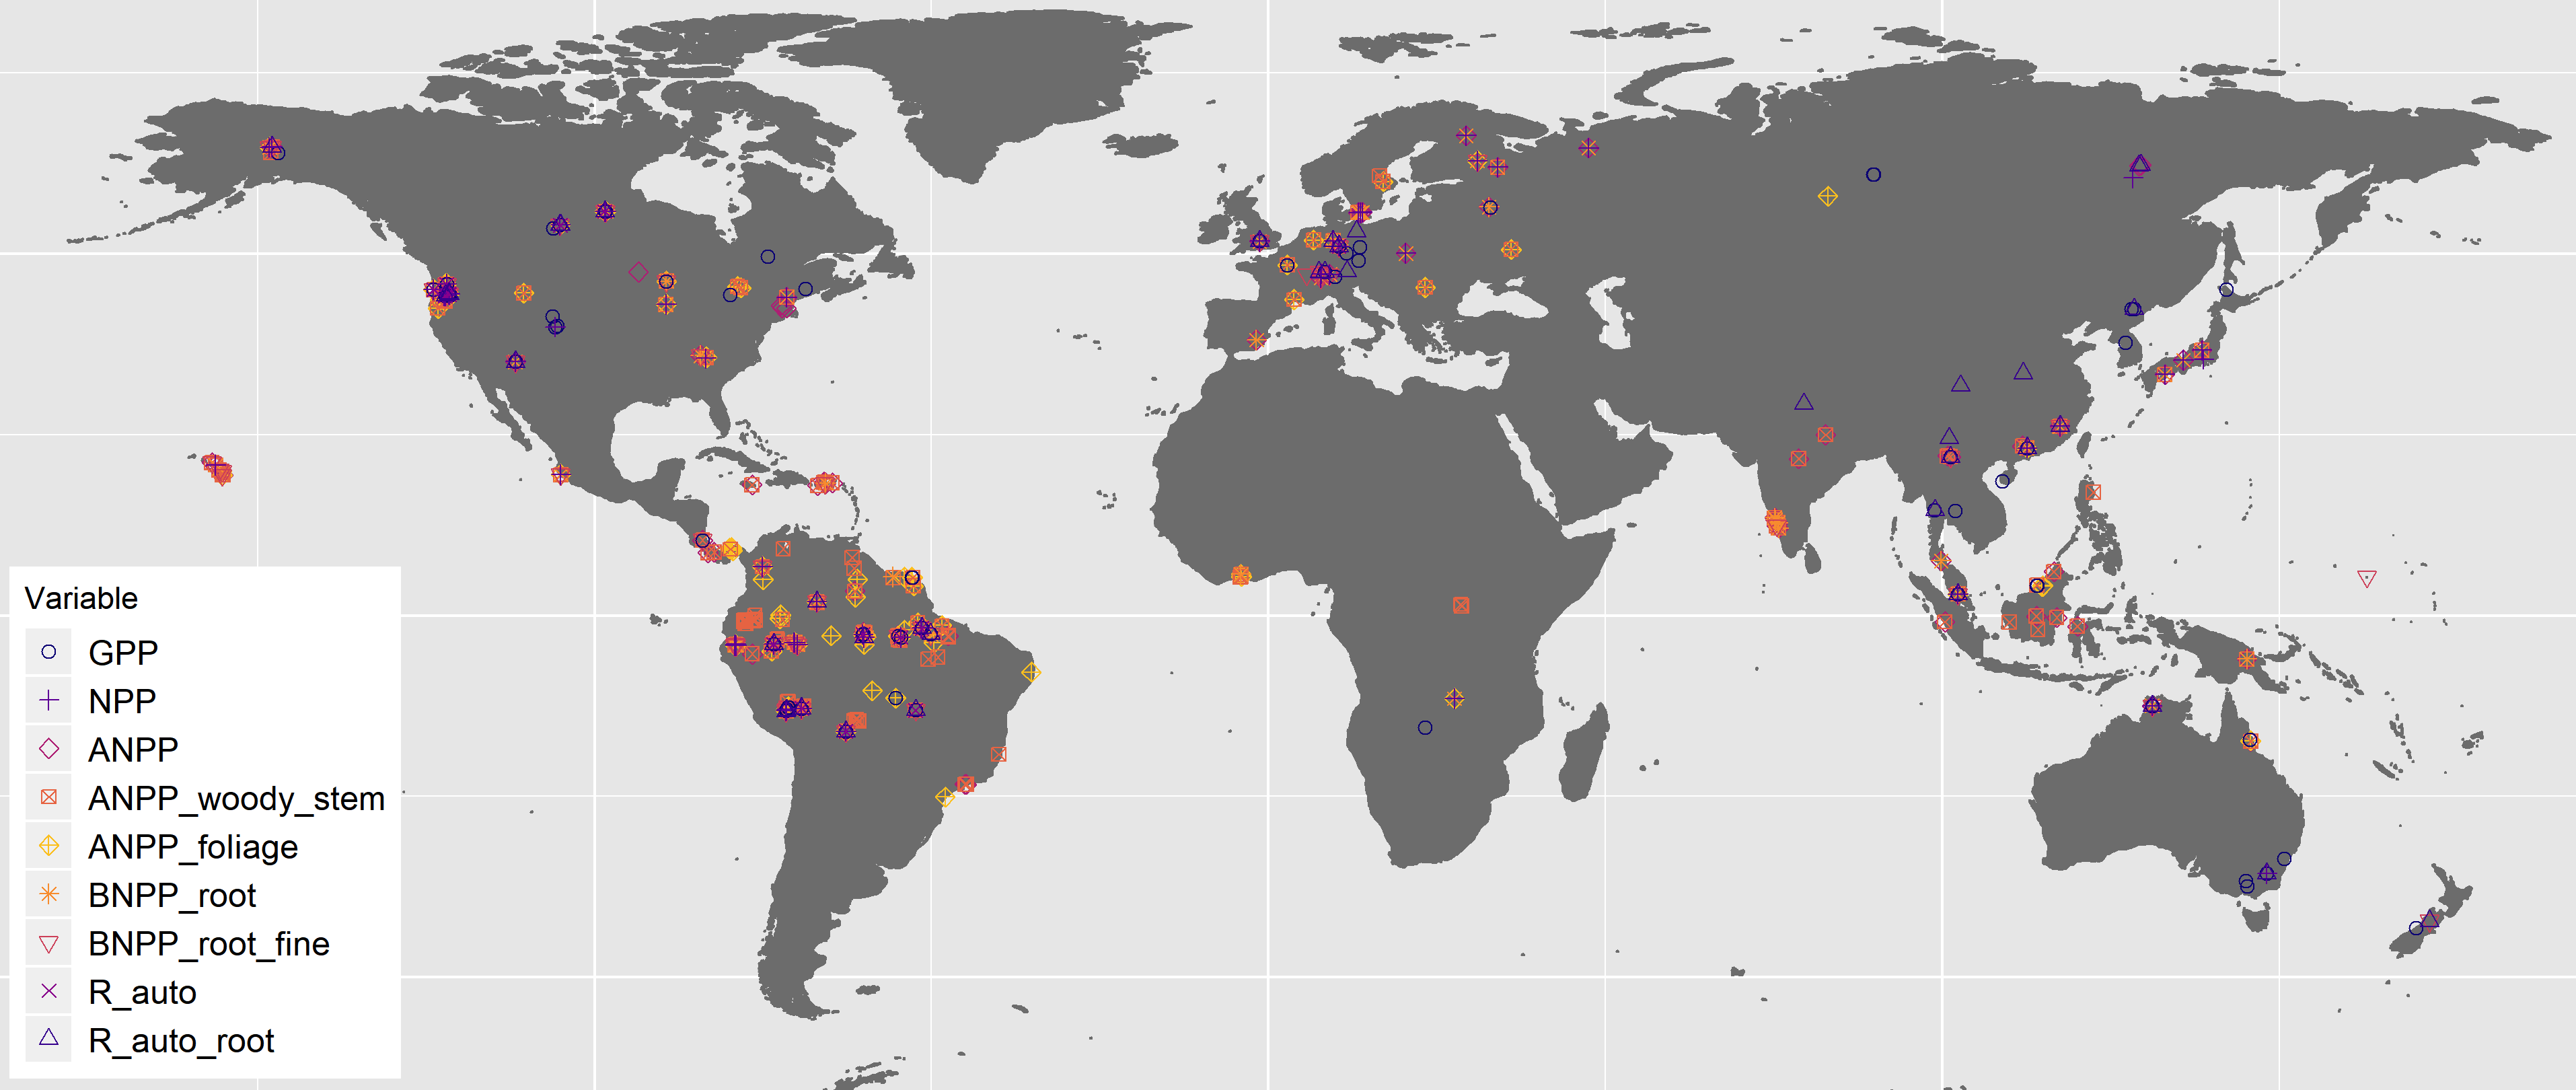
\includegraphics[width=1\linewidth]{distribution_all_variables_cropped} \caption{Map showing all data used in the analysis, coded by variable. Variables are plotted individually in Fig. S1. }\label{fig:unnamed-chunk-6}
\end{figure}

\emph{Climate data}

ForC contains geographic coordinates associated with each measurement
record and, when available, mean annual temperature (MAT) and mean
annual precipitation (MAP) as reported in the primary literature
\citep{anderson-teixeira_forc_2018}. Based on the geographic
co-ordinates for each site, data on twelve climate variables--including
MAT, MAP, temperature and precipitation seasonality, annual temperature
range, solar radiation, cloud cover, annual frost and wet days,
potential evapotranspiration (PET), aridity (MAP/PET), and vapor
pressure deficit (VPD)--were extracted from five open-access climate
datasets: WorldClim \citep{hijmans_very_2005}, WorldClim2
\citep{fick_worldclim_2017}, the Climate Research Unit time-series
dataset (CRU TS v4.03 \citep{harris_updated_2014}, the Global Aridity
Index and Potential Evapotranspiration Climate Database
\citep{trabucco_global_2019}, and TerraClimate
\citep{abatzoglou_terraclimate_2018} (Table S1). From these data, we
derived maximum VPD, defined as the VPD of the month with the largest
deficit, and the number of water stress months, defined as the number of
months annually where precipitation was lower than PET. Where site-level
data was missing for MAT or MAP, we used values from the WorldClim
dataset.

\textbf{For consistency with previous studies (Table 1, \emph{H5}),}
length of the growing season was estimated to the nearest month, where
growing season months were defined as months with mean minimum
temperature \textgreater{} 0.5\(^\circ\)C. We experimented with a
definition of growing season months including a moisture index, defined
as (MAT - PET)/PET, \textgreater{} -0.95
\citetext{\citealp{kerkhoff_plant_2005}; \citealp[see
also][]{michaletz_convergence_2014}}. However, we found that including a
moisture index had minimal effect on the estimates of growing season
length, and so chose to exclude it. Monthly data for PET, precipitation,
and temperature from CRU v 4.03 \citep{harris_updated_2014} and solar
radiation from WorldClim2 \citep{fick_worldclim_2017} were used to
calculate mean monthly PET, precipitation, temperature and solar
radiation during the growing season. Total growing season precipitation
and solar radiation were also calculated.

\emph{Analyses}

The effects of latitude and climate on C fluxes were analysed using
mixed effects models using the package `lme4' \citep{bates_fitting_2015}
in R v.3.5.1 \citep{r_core_team_r:_2018}. The basic model for all
analyses included a fixed effect of latitude or climate and a random
effect of plot nested within geographic area. Geographic
areas--\emph{i.e.}, spatially clustered sites--are defined within ForC
using a hierarchical cluster analysis on the distance matrix of the
sites and a cutoff of 25km \citep{anderson-teixeira_forc_2018}. We
experimented with inclusion of altitude as a fixed effect, but excluded
it from the final models because it added very little explanatory
power--that is, the difference in AIC (\(\Delta\) AIC) relative to
models excluding altitude was generally small (often \(\Delta\)
AIC\textless2). Effects were considered significant when inclusion of
the fixed effect of interest resulted in p \(\le\) 0.05 and \(\Delta\)
AIC \(\ge\) 2.0 relative to a corresponding null model. All \(R^2\)
values presented here are marginal \(R^2\) values, and refer to the
proportion of variation explained by only the fixed effects. Specific
analyses are as described below.

We first examined the relationship between latitude and C fluxes
(\emph{Q1}; Table 1). We tested models with latitude as a first-order
linear, second-order polynomial, and logarithmic term. For brevity, we
henceforth refer to first-order linear models as ``linear'' and
second-order polynomial models as ``polynomial''. We selected as the
best model that with the highest \(\Delta\) AIC relative to a null model
with no fixed term, with the qualification that a polynomial model was
considered an improvement over a linear model only if it reduced the AIC
value by 2.0 or more.

To test whether trends in component fluxes across latitude sum to match
those of larger fluxes, regression lines for smaller component fluxes
were summed to generate new estimates of larger fluxes. Because no
fluxes were significantly better predicted by a logarithmic or
polynomial fit than by a linear fit, we used linear fits for all fluxes.
We then determined whether these summed predictions fell within the 95\%
CI for the larger flux across the entire latitudinal range. Confidence
intervals for the line of best fit for the larger flux were estimated
using the `bootMer' function, a parametric bootstrapping method for
mixed models \citep{bates_fitting_2015}. This function carried out 2000
simulations estimating the line of best fit, using quantiles at 0.025
and 0.975 to estimate 95\% CIs. This analysis was applied to the
following sets of fluxes: (1) \(GPP = NPP + R_{auto}\), (2)
\(NPP = ANPP + BNPP\), and (3) \(ANPP = ANPP_{foliage} + ANPP_{stem}\).
In addition, we estimated total belowground C flux (TBCF, not analyzed
due to limited data) as \(TBCF = BNPP + R_{root}\).

Variation in allocation to component carbon fluxes was explored for
three groupings: (1) \(GPP = NPP + R_{auto}\), (2)
\(NPP = ANPP + BNPP\), and (3) \(ANPP = ANPP_{foliage} + ANPP_{stem}\).
For each group, measurements taken at the same site and plot, an in the
same year were grouped together. For groups (1) and (2), where 2 of the
3 flux measurements were available for a given site, plot, and year,
these measurements were used to calculate the third. The ratio of each
pair of component fluxes was calculated. The log of these ratios were
regressed against latitude and climate variables, using the linear model
specified above. Cook's distance analyses were carried out for each of
the models, and extreme outliers removed,

We next examined the relationships of C fluxes to climate variables
(Q2-Q4; Table 1). We tested first-order linear, second-order polynomial,
and logarithmic fits for each climate variable. Again, polynomial fits
were considered superior to first-order linear fits only if inclusion of
a second-order polynomial term resulted in \(\Delta\) AIC \(\ge\) 2.0
relative to a first-order linear model. We tested relationships of each
C flux (Table 2) against each climate variable (Table S1). Variables
which were not significant explanatory variables or which explained
\textless20\% of variation in C fluxes are only presented in SI.

Multivariate models were used to investigate the potential joint and
interactive effects of MAT and MAP on carbon fluxes. An additive model
including MAP in addition to MAT was accepted when \(\Delta\) AIC
\textgreater2 relative to a null including only MAT as a fixed effect.
An interactive model including an MAT x MAP interaction was accepted
when \(\Delta\)AIC \textgreater2 relative to a null including MAT and
MAP as fixed effects.

To test whether and how C flux varied with climate when standardised by
growing season length (Q5), we first standardized all annual C fluxes by
dividing by growing season length (as defined above). We then derived
four variables to describe growing season climate, specifically growing
season temperature, precipitation, solar radiation, and PET (Table S1).
We tested for correlations between these standardised fluxes and growing
season climate variables, using only first-order linear models.

\textbf{All analyses were conducted in R (}Version\textbf{). Code and
data necessary to reproduce all results are archived on GitHub\ldots.}

\#\#\#Results

In total, we analyzed 1319 records from nine forest autotrophic C flux
variables taken from forests that had experienced no major anthropogenic
disturbances within the past 100 years. These records represented a
total of 255 plots in 154 distinct geographic areas across all forested
biogeographic and climate zones (Fig. 1, Table 2).

\emph{How does C flux vary with latitude?}

All major carbon fluxes decreased with latitude (Fig. 2; Table S2).
Latitude was a strong predictor for many of the carbon fluxes,
particularly the larger fluxes (Table S2). Specifically, latitude
explained 64\% of variation in GPP (n = 243, p\textless0.0001), 50\% in
NPP (n = 161, p\textless0.0001) and 44\% in ANPP (n = 278,
p\textless0.0001). The C fluxes that were most poorly predicted by
latitude were \(BNPP_{fine.root}\) (\(R^2\)=0.17) and \(ANPP_{stem}\)
(\(R^2\)=0.18). The relationship with latitude was best fit by the
first-order linear model, with the exception of NPP and \(R_{root}\),
for which a logarithmic model was a slightly - but not significantly -
better fit.

\begin{figure}[H]
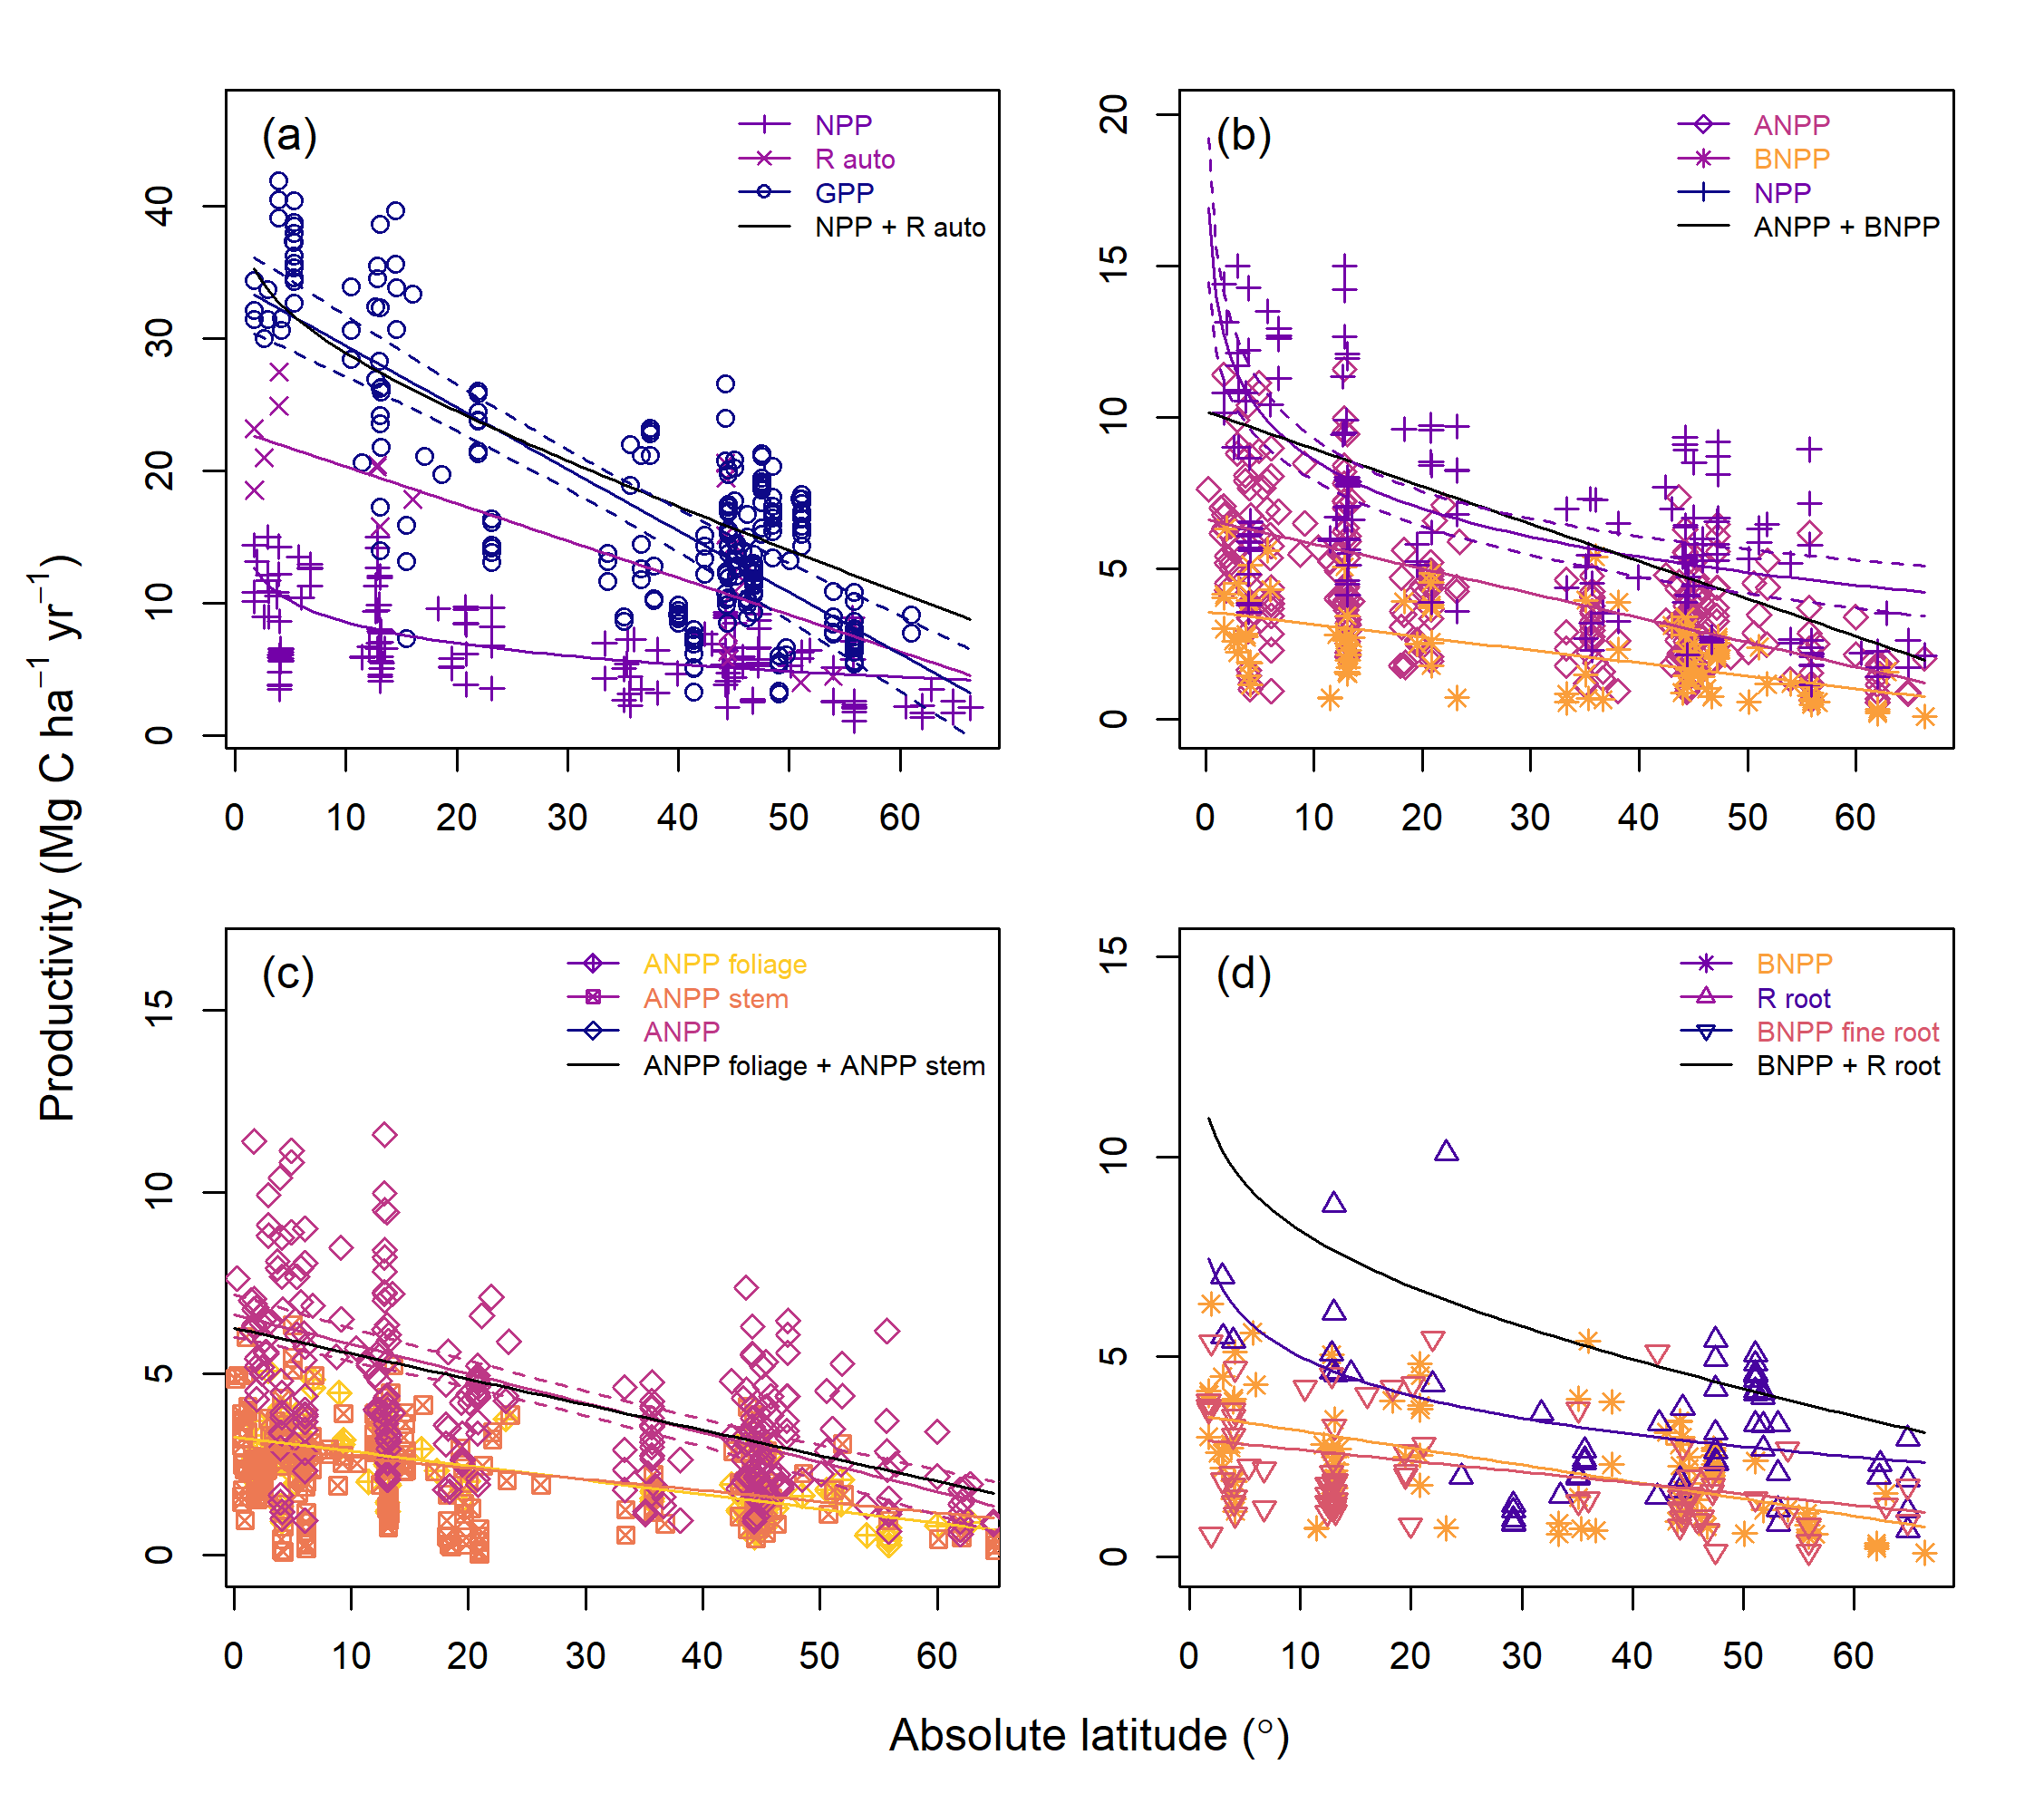
\includegraphics[width=1\linewidth]{combined_stacked} \caption{Latitudinal trends in forest autotropic carbon flux. Plotted are linear models, all of which were significant $(p<0.05)$ and had AIC values within 2.0 of the best model (for two fluxes, logarithmic fits were marginally better; Table S2). Each panel shows major C fluxes together with component fluxes. Also plotted are predicted trends in the major C fluxes based on the sum of component fluxes. 95\% confidence intervals are plotted for the major flux for comparison with predicted trends. In (d), which shows three belowground fluxes, the major flux, total belowground carbon flux, has insufficient data (n=9) to support a regression}\label{fig:unnamed-chunk-7}
\end{figure}

In general, smaller component fluxes summed approximately to larger
fluxes across the latitudinal gradient (Fig. 2). That is, modeled
estimates of \(GPP\), generated from the sum of \(NPP\) and
\(R_{auto}\); \(NPP\), generated from the sum of \(ANPP\) and \(BNPP\);
and \(ANPP\), generated from the sum of \(ANPP_{foliage}\) and
\(ANPP_{stem}\), fell almost completely within the confidence intervals
of the regressions of field estimates of \(GPP\), \(NPP\), and \(ANPP\),
respectively.

We found no evidence of systematic variation in C allocation with
latitude or climate (Fig. S3). Of 12 relationships tested (3 ratios
among C flux variables regressed against latitude, MAT, MAP and
temperature seasonality), none were significant.

\emph{How does C flux relate to MAT and MAP?}

All fluxes increased with MAT (all p\textless0.05; Figs. 3-4, S4-S5,
Table S2). For eight of the nine fluxes, this relationship was linear.
For only one variable, \(BNPP\), did a lognormal fit provide signficant
improvement over a first-order linear relationship. \emph{As with
latitude, MAT tended to explain more variation in the larger fluxes
(\(GPP\), \(NPP\), \(ANPP\), \(R_{auto}\)) and \(ANPP_{foliage}\) (all
\(R^2\)\textgreater{} 0.4) than in subsidiary and belowground fluxes
(\(ANPP_{stem}\), \(R_{root}\), \(BNPP_{fine.root}\); all
\(R^2\)\textless{} 0.25).} \textbf{update this -- NB these values are
correct}

MAP was a significant (p\textless0.05) predictor of all fluxes (Figs.
4a, S4-S5; Table S2). However, it explained little variation: with the
exception of \(R_{auto}\), MAP explained at most 25\% of variation in C
flux. All fluxes increased with MAP up to at least 2000 mm, above which
responses were variable (Figs. 4, S4-S5).\\
There was a significant additive effect of MAT and MAP on \(GPP\),
\(ANPP\) and \(R_{auto}\) (Fig. 3, Table S3), and a significant
interactive effect between MAT and MAP for \(NPP\) and \(ANPP_{stem}\)
(Fig. 3, Table S3). The interaction was negative for \(NPP\) and
positive for \(ANPP_{stem}\). For \(ANPP_{foliage}\), \(BNPP\),
\(BNPP_{fine.root}\), and \(R_{root}\), MAP did not have a signficant
effect when accounting for MAT (Fig. 3, Table S3).

\begin{figure}[H]
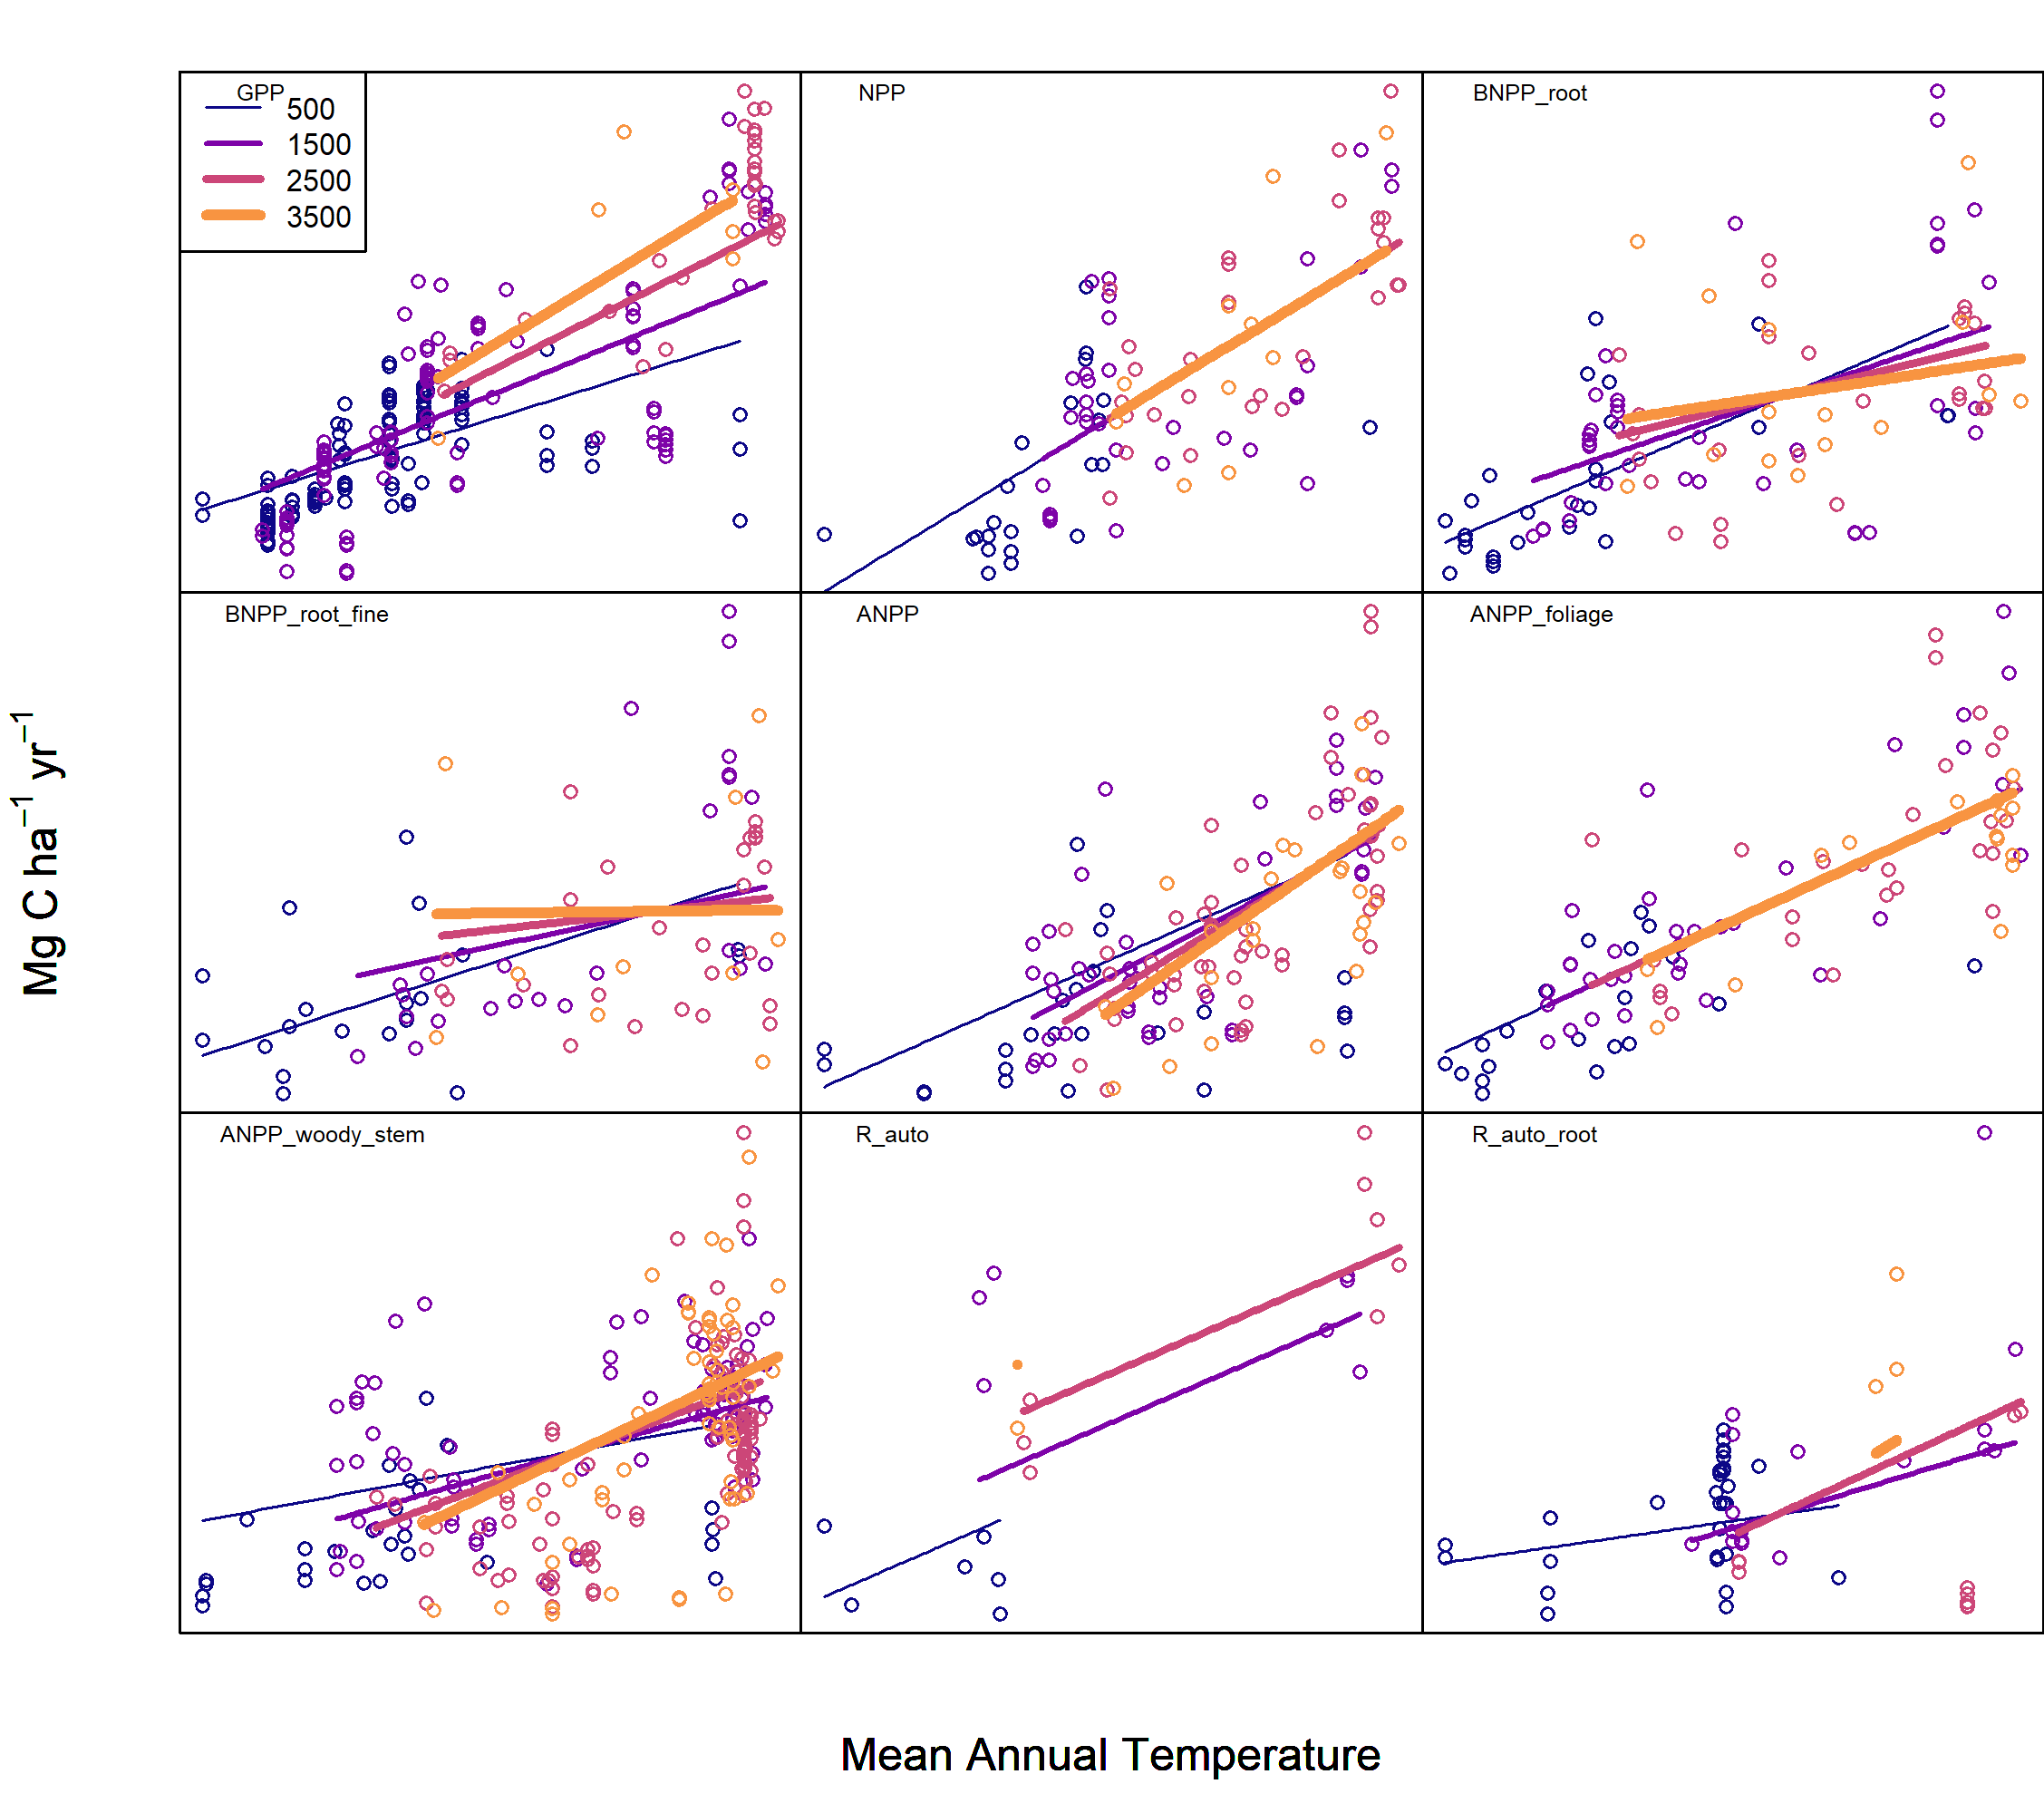
\includegraphics[width=1\linewidth]{mat_map_interaction} \caption{Interactive effects of mean annual temperature and precipitation on annual forest carbon fluxes. For visualization purposes, data points are grouped into bins of 0 - 1000, 1001 - 2000, 2001 - 3000, and >3000mm mean annual precipitation, and lines of best fit models are plotted for mean annual precipitation values of 500, 1500, 2500, and 3500mm. All regressions are significant $(p<0.05)$.}\label{fig:unnamed-chunk-8}
\end{figure}

\emph{How does C flux relate to other climate variables?}

Our results indicated that annual forest C fluxes were most strongly
explained by temperature-related climate variables at the global scale.
In addition to MAT, several of its correlates (Fig. S2) were
consistently identified as strong univariate predictors of C fluxes:
temperature seasonality, annual temperature range, annual frost days,
PET, and length of growing season (Figs. 4, S4-S7).

All C flux variables showed a significant relationship with potential
evapotranspiration. The relationship was logarithmic for
\(ANPP_{foliage}\), \(BNPP_{fine.root}\) and \(R_{root}\), and
polynomial for all other fluxes (Fig. 4c, S4-5; Table S2). We found
strong evidence for a saturation point or peak with PET: C fluxes tended
to increase at values below 1000mm, before saturating between 1200 and
1700mm. There was also evidence that some C fluxes begin to decrease at
values above 1800mm PET.

Vapour pressure deficit was a significant predictor of all C fluxes.
\(ANPP_{foliage}\), \(BNPP_{fine.root}\) and \(R_{root}\) showed a
logarithmic relationship with vapour pressure deficit, but all other
fluxes showed a polynomial relationship (Figs. 4d, S4-5; Table S2). C
fluxes initially increased with vapour pressure deficit, before
saturating at around 0.8 kPa, after which point they began to decrease.

All fluxes, with the exception of \(R_{root}\), showed a significant
positive relationship with solar radiation (Figs. S4-S5, Table S2).
Solar radiation explained a low proportion of variability in all C
fluxes, explaining less than 30\% of the variation in each flux

Annual wet days, cloud cover, aridity, and water stress months were poor
or non-significant explainers of variation in C fluxes, explaining less
than 20\% of the variation in each of the carbon fluxes (Figs. S4-S5;
Table S2).

\begin{figure}[H]
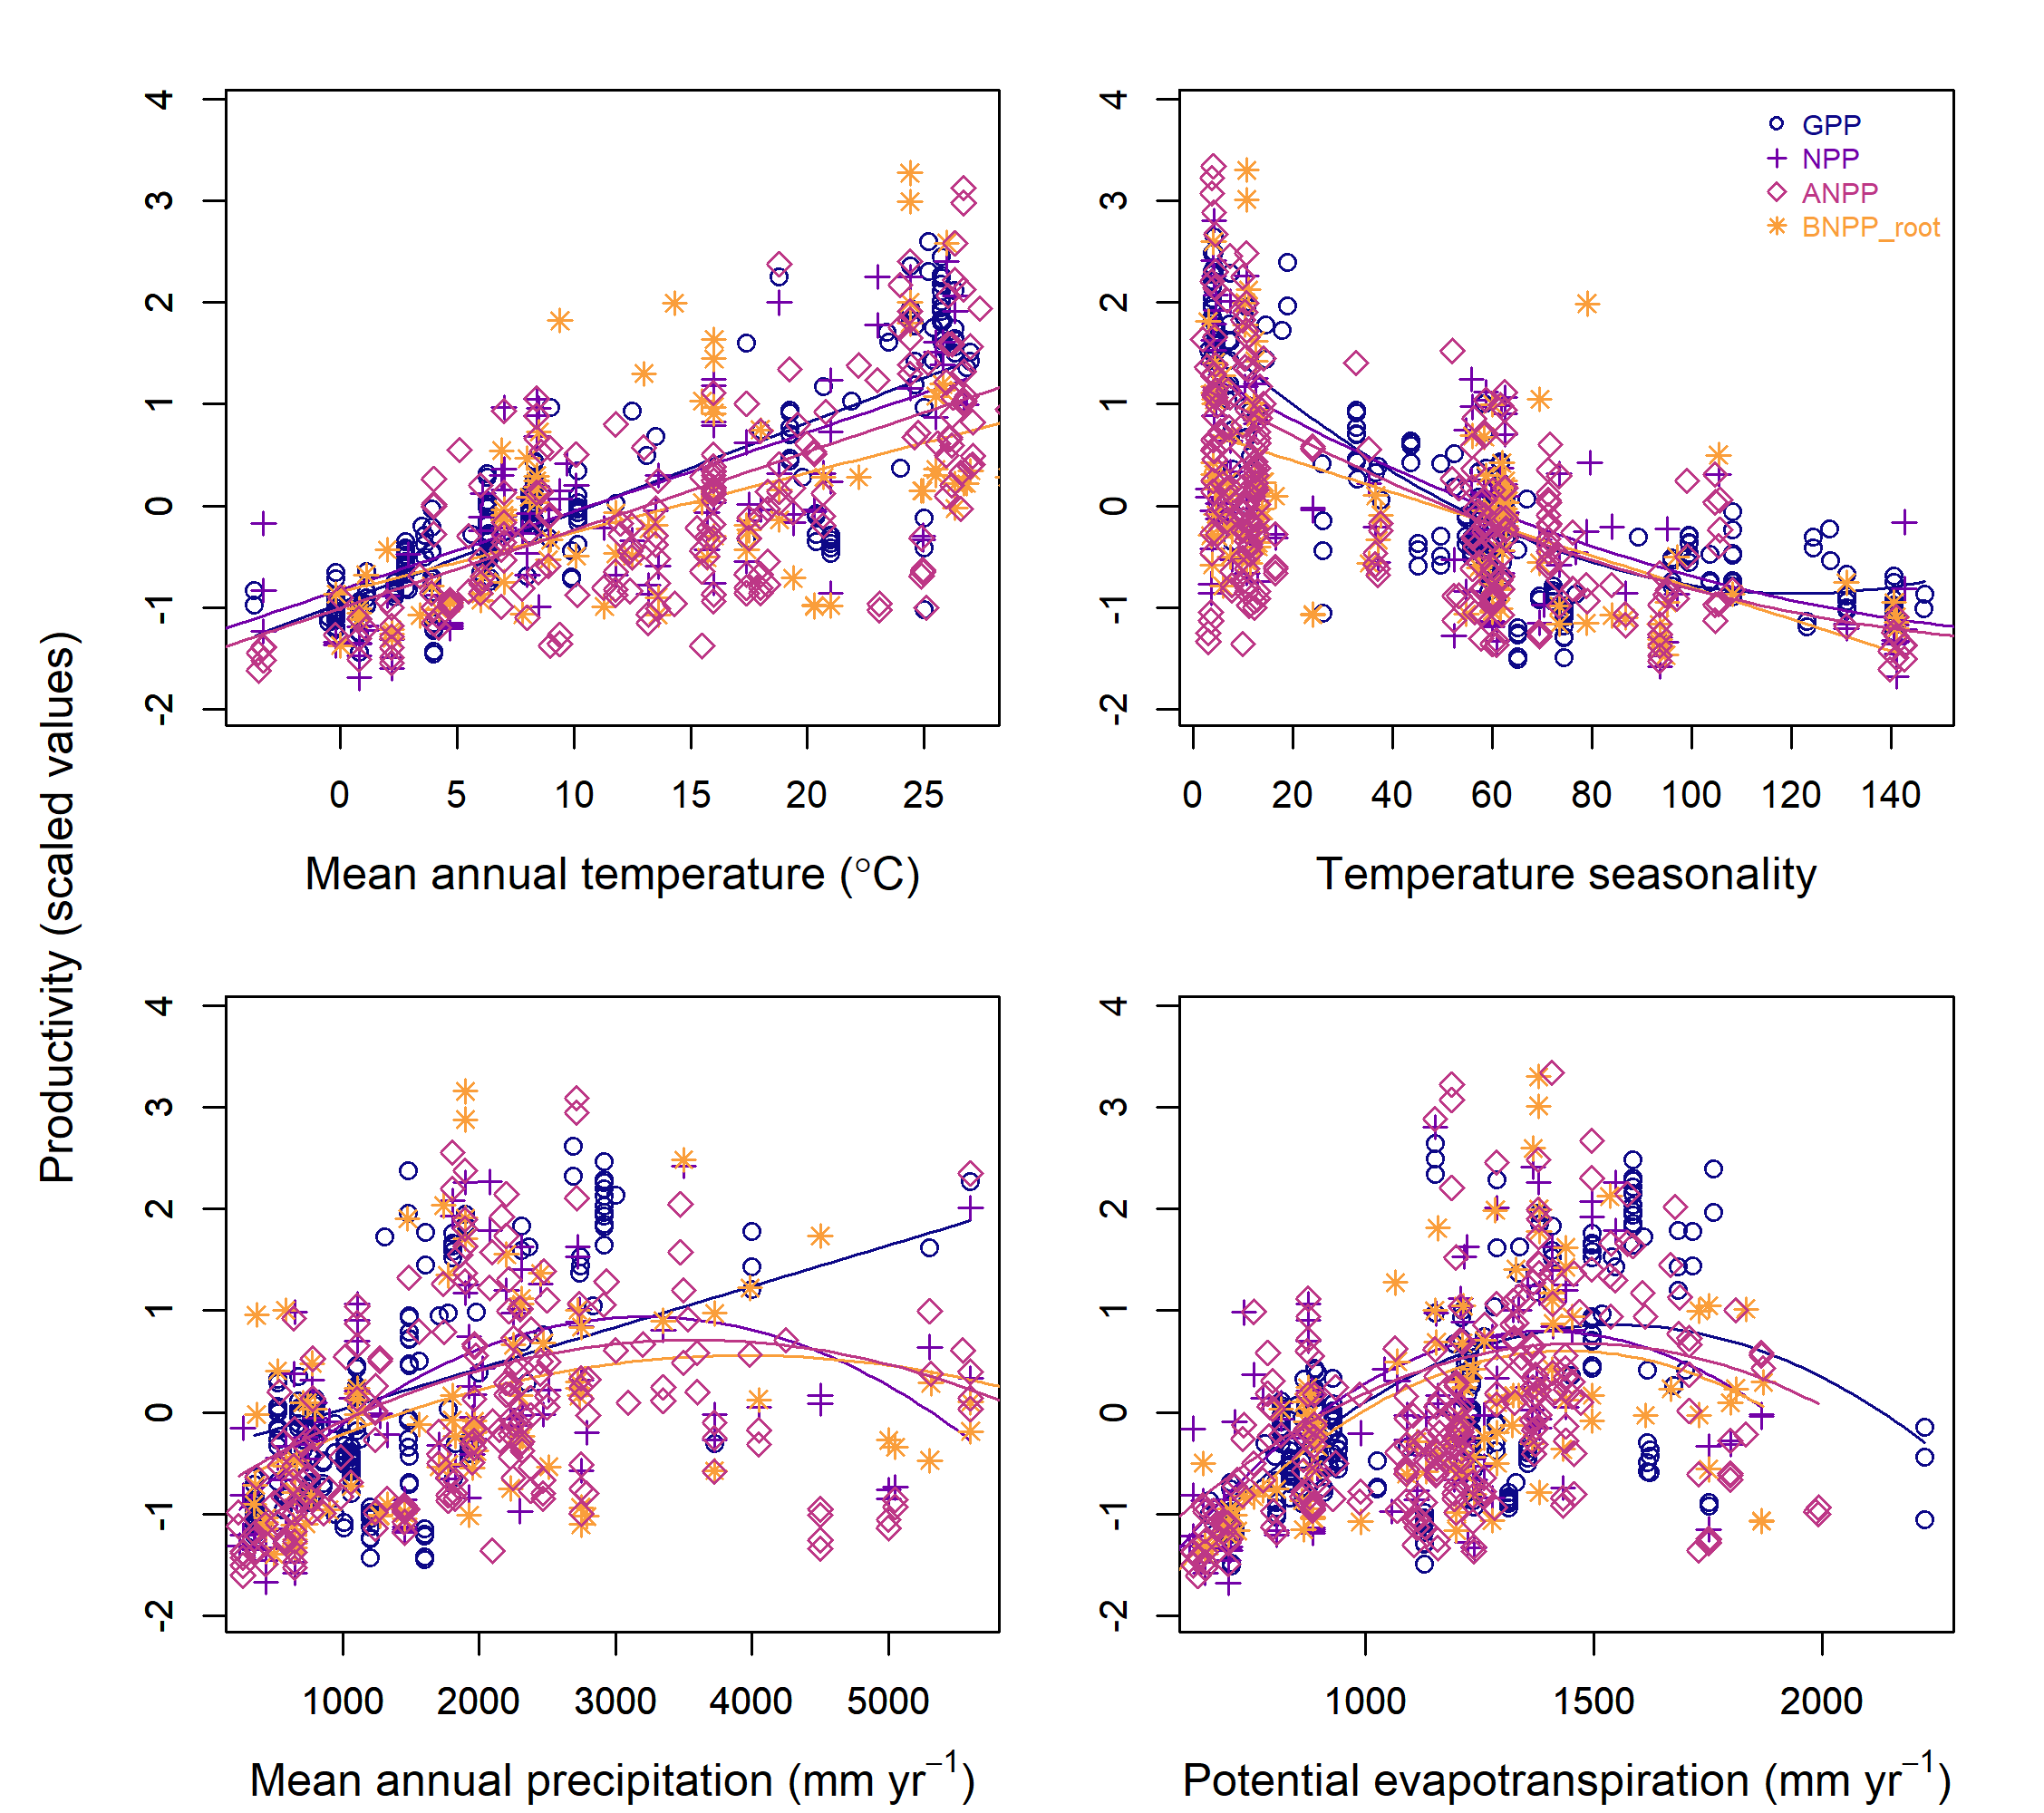
\includegraphics[width=1\linewidth]{combined_plots} \caption{Plots of carbon fluxes against (a) mean annual temperature; (b) mean annual precipitation; (c) potential evapotranspiration, (d) vapour pressure deficit; (e) temperature seasonality; (f) length of growing season. For visualization purposes, data for each flux was rescaled with a mean of 0 and standard deviation of 1. Lines of best fit are plotted according to the best model selected during analysis (**see issue 47**). All regressions are significant $(p<0.05)$.}\label{fig:unnamed-chunk-9}
\end{figure}

\emph{What is the role of seasonality in explaining C fluxes?}

Temperature seasonality was a strong predictor of annual C fluxes. All
fluxes decrease with increasing seasonality, though the shape of this
relationship varies (all p\textless0.05; Figs. 4e, S6-7; Table S2).
Temperature seasonality was strongly correlated with annual temperature
range, which was likewise a similarly strong predictor of C fluxes
(Table S2). C fluxes were highest where temperature seasonality = 0, and
at an annual temperature range of 15\(^\circ\)C or lower. \textbf{BBL:
perhaps put this into an ecosystem context; what are these? Aseasonal
subtropical places?}

In contrast, there was no significant effect of precipitation
seasonality on C fluxes, and both maximum vapour pressure deficit, and
water stress months were poor or non-significant predictors of variation
in C fluxes (Figs. S6-S7; Table S2).

We found a significant relationship between length of growing season and
C fluxes, with all fluxes showing a positive relationship with length of
growing season (Figs. 4e, S6-S7; Table S2). Length of growing season was
a strong predictor of C fluxes, explaining 53\% of variation in GPP,
38\% of variation in NPP, and 34\% of variation in ANPP (all
p\textless0.05; Table S2), but it was a weaker predictor than MAT for
all fluxes analysed (Table S4).

\emph{Within the growing season, how do C fluxes vary with climate?}

When annual C fluxes were standardized by growing season length (in
monthly increments), correlations with growing season climate were
generally weak (Figs. S8-S9). \(ANPP\) increased with growing season
temperature (\(R^2\) = 0.09, p\textless0.001) and precipitation (\(R^2\)
= 0.04, p\textless0.05). Similarly, \(ANPP_{foliage}\) increased
slightly with growing season temperature (\(R^2\) = 0.16,
p\textless0.01) and precipitation (\(R^2\) = 0.09, p\textless0.05).
Growing season solar radiation had a positive influence on \(BNPP\)
(\(R^2\) = 0.17, p\textless0.001) and \(BNPP_{fine.root}\) (\(R^2\) =
0.13, p\textless0.01). Growing season PET had a positive influence on
\(GPP\) (\(R^2\) = 0.15, p\textless0.01), \(NPP\) (\(R^2\) = 0.07,
p\textless0.01), \(BNPP\) (\(R^2\) = 0.23, p\textless0.0001),
\(BNPP_{fine.root}\) (\(R^2\) = 0.10, p\textless0.05), and
\(ANPP_{stem}\) (\(R^2\) = 0.06, p\textless0.05). All other
relationships were non-significant.

\#\#\#Discussion

Our analysis of a large global database (ForC) clarifies how autotrophic
C fluxes in mature forests vary with latitude and climate on a global
scale. We show that, across all nine variables analyzed, annual C flux
decreases continually with latitude (Fig. 2)--a finding that confirms
multiple previous studies but contradicts the idea that productivity of
temperate forests rivals or even exceeds that of tropical forests
\citep{luyssaert_co_2007, huston_global_2009}. At this global scale, C
fluxes increase approximately in proportion to one another, with
component fluxes summing appropriately to larger fluxes and no
detectable differences in allocation across latitude or climates (Figs.
2, 4, S3). Similarly, we show broad - \emph{albeit} not complete -
consistency of climate responses across C fluxes, with the observed
latitudinal variation primarily attributable to temperature and its
seasonality (Figs. 3-4). Water availability is also influential, but of
secondary importance across the climate space occupied by forests (Figs.
3-4). Contrary to prior suggestions that the majority of variation in C
cycling is driven by the length of the growing season (\textbf{REFS}),
we find modest explanatory power of growing season length and small but
sometimes significant influence of climate within the growing season
(Figs. 4f,S6-S9). Together, these findings yield a unified understanding
of climate's influence on forest C cycling.

Our findings indicate that, among mature, undisturbed stands, forest C
fluxes are unambiguously highest in the tropical regions, and the
relationship with both latitude and \(MAT\) is approximately linear
(Figs. 2, 4). This contrasts with the suggestion that C fluxes (e.g.,
\(NPP\), \(ANPP\), \(ANPP_{stem}\)) of temperate forests are similar to
or even greater than that of tropical forests
\citep{luyssaert_co_2007, huston_global_2009}. Previous indications of
such a pattern may have been an artifact of differences in stand age
across biomes. Compared to tropical forests, the temperate forest biome
has experienced more widespread anthropogenic disturbance and has a
larger fraction of secondary stands
\citep{potapov_mapping_2008, poulter_global_2018}, so analyses comparing
across latitudinal gradients without controlling for stand age risk
confounding age with biome effects. Because carbon allocation varies
with stand age
\citep{de_lucia_forest_2007, anderson-teixeira_altered_2013, doughty_what_2018},
age differences may introduce systematic biases into analyses of C
fluxes across latitude or global climatic gradients. For example, woody
productivity tends to be higher in rapidly aggrading secondary stands
than in old-growth forests, where proportionally more C is allocated to
respiration and non-woody productivity
\citep{de_lucia_forest_2007, piao_forest_2010, doughty_what_2018, kunert_understanding_2019}.
Thus, findings that temperate forest productivity rivals that of
tropical forests are likely an artifact of different forest ages across
biomes.

We show that C fluxes are broadly consistent in their responses to
climate drivers on the global scale, with no trends in C allocation
among the variable pairs tested (Figs. 2, 4, S3). This parallels the
observation that C allocation across multiple C fluxes varies little
with respect to climate along a steep tropical elevational gradient
\citetext{\citealp{malhi_variation_2017}; \citealp[but
see][]{moser_elevation_2011}}, and is not surprising given that carbon
allocation within forest ecosystems is relatively constrained
\citep{enquist_global_2002, litton_carbon_2007, malhi_allocation_2011}.
We find no trend in the allocation of \(GPP\) between production and
respiration across latitude or climate (\(NPP\):\(R_{auto}\); Fig. S3),
refuting the idea that tropical forests have anomalously low \(CUE\)
\citep{de_lucia_forest_2007, malhi_productivity_2012, anderson-teixeira_carbon_2016}.
Rather, differences in \(CUE\) between old-growth tropical forests
relative to (mostly younger) extratropical forests are likely an
artifact of comparing stands of different age, as \(CUE\) is known to
decline with forest age
\citep{de_lucia_forest_2007, piao_forest_2010, collalti_is_2019}.
Another previously observed pattern for which we find no support is a
tendency for belowground C allocation to decrease with increasing
temperature \citep{moser_elevation_2011, gill_belowground_2016}; rather,
we observe no trends in allocation between \(ANPP\) and \(BNPP\) across
latitudes. Failure to detect signficant tends in C allocation with
respect to climate in this analysis does not imply that none exist;
rather, it suggests that

Despite the broad consistency of climate responses across C fluxes,
climate explains lower proportions of variability among some of the
subsidiary C fluxes (\emph{e.g.}, \(ANPP_{stem}\), \(BNPP\)
\(BNPP_{fine.root}\); Fig. 2; Tables S2, S6). There are two,
non-exclusive, potential explanations for this. First, it may be that
methodological variation is larger relative to flux magnitude for some
of the subsidiary fluxes. Belowground fluxes in particular are difficult
to quantify, and measurement methods for the belowground fluxes
considered here may use fundamentally different approaches in different
sites (\emph{e.g.}, minirhizotrons, ingrowth cores, or sequential coring
for \(BNPP_{fine.root}\); root exclusion, stable isotope tracking, or
gas exchange of excised roots for \(R_{root}\)), and sampling depth is
variable and often insufficient to capture the full soil profile.
\(ANPP_{stem}\), which is also poorly explained by latitude or climate,
is more straightforward to measure but is subject to variability
introduced by differences such as biomass allometries applied and
minimum plant size sampled \citep{clark_measuring_2001}. However,
methodological variation and uncertainty affect all of fluxes considered
here, and some of the larger fluxes that vary more strongly with respect
to climate (\(ANPP\), \(NPP\)) are estimated by summing uncertain
component fluxes. Second, differences among variables in the proportion
of variation explained by climate may be attributable to more direct
climatic control over \(GPP\) than subsidiary fluxes. That is,
subsidiary fluxes may be shaped by climate both indirectly through its
influence on \(GPP\) and respiration and directly through any climatic
influence on C allocation, as well as many other local- and
regional-scale factors \citep[e.g.,][]{moser_elevation_2011}
(\textbf{REFS-BECKY, know any?}).

Temperature and its seasonality were the primary drivers of C flux on
the global scale (Figs. 2-4), consistent with a long legacy of research
identifying temperature as a primary driver of forest ecosystem C
cycling
\citep[e.g.,][]{lieth_primary_1973, luyssaert_co_2007, wei_forest_2010}.
We find little evidence of any non-linearity in temperature's influence
on C flux. The relationship of all fluxes to \(MAT\) as an individual
driver were best described by a linear function (Table S2) - with the
exception of \(BNPP\), whose response to \(MAT\) was close to linear
(Fig. 4a). This result contrasts with the idea that fluxes saturate with
\(MAT\) below approximately 25\(^\circ\)C \(MAT\)
\citep{luyssaert_co_2007, huston_global_2009}. It remains possible that
flux declines above this threshold
\citep{larjavaara_temperature_2012, sullivan_long-term_2020}, as is also
consistent with tree-ring records indicating that tropical tree growth
declines at high temperatures \citep[e.g.,][]{vlam_temperature_2014}.
However, these higher temperatures also tend to be associated with high
PET and VPD, both of which are associated with reduced C fluxes (Figs.
4c-d, S4-S5). Indeed, while temperature responses dominate at this
global scale and with the climate space occupied by forests, the effects
of temperature are moderated by moisture availability (Table 1; Figs
3-4). Specifically, C fluxes are reduced under relatively dry conditions
(\emph{i.e.}, low \(MAP\); high \(VPD\)) and sometimes under very high
precipitation (Figs. 3-4). The observed positive interaction between
\(MAT\) and \(MAP\) for \(ANPP_{stem}\) on the global scale (Fig. 3) is
consistent with an analysis showing a similar interaction for \(ANPP\)
in tropical forests, also with a cross-over point at
\textasciitilde20\(\circ\)C \citep{taylor_temperature_2017}.\\
However, we detect no such interaction for \(ANPP\) or most other C
fluxes, and we find a contrasting negative interaction for \(NPP\) (Fig.
3), suggesting that more data are required to sort out potential
differences in the interactive effects of MAT and MAP on C fluxes in the
tropics.

Forest autotrophic C fluxes decline with temperature seasonality (Table
1, \emph{H4}; Fig. 4e), and are minimal during cold- or dry- dormant
seasons. To account for this, a number of analyses seeking to
characterize global-scale effects of climate on productivity have
examined the relationship of C flux per month of the growing season with
growing season climatic conditions \citep[Table 1,
\emph{H5};][]{kerkhoff_plant_2005, anderson_temperature-dependence_2006, enquist_adaptive_2007, michaletz_convergence_2014}.
The sort of simple metric that has been used to define growing season at
a global scale \citep{kerkhoff_plant_2005} is coarse with respect to
temperature because it is calculated on a monthly timescale and
problematic with respect to moisture because it doesn't capture temporal
lags between precipitation and plant water use caused by storage in soil
or snow. We found that a temperature-defined growing season length had
strong positive correlation with C fluxes (Fig. 4f), but was never the
best univariate predictor. Dividing annual fluxes by growing season
length to yield average flux per growing season month removed the
majority of climate-related variation, supporting the idea that the
latitudinal gradient in carbon flux is attributable more to shorter
growing seasons at high latitudes than to inherently lower rates of
photosynthesis or respiration by high-latitude forests
\citep{enquist_adaptive_2007}. However, there remained a number of
significant correlations with growing season climatic conditions,
indicating that climatic conditions remain influential within the
growing season (Figs. S8-S9). We conclude that while correcting for
growing season length takes analyses a step closer to mechanistic
linkage of instantaneous C flux rates to environmental conditions, it
remains crude relative to the timescales on which climate affects plant
metabolism, and does not advance statistical predictive power.
Mechanistic accounting for climatic effects on global forest carbon flux
patterns instead requires models representing physiologically meaningful
timescales
\citep[e.g.,][]{medvigy_mechanistic_2009, longo_biophysics_2019}.

Our analysis clarifies how forest autotrophic carbon fluxes vary with
latitude and climate on a global scale, with some important implications
for how forest carbon cycling relates to climate and, by extension, how
it is likely to respond to climatic warming. To the extend that patterns
across broad scale climatic gradients can foretell how ecosystem
responses to climate change, our findings suggest that higher
temperatures with similar moisture availability result in a generalized
acceleration of forest C cycling (Figs. 2-3). This is consistent with
observations of continental- to global-scale increases over time in
\(GPP\) \citep{li_mapping_2019} and \(ANPP_{stem}\)
\citep{brienen_long-term_2015, hubau_asynchronous_2020}, along with some
C cycle components not considered here--tree mortality
\citep{brienen_long-term_2015, mcdowell_drivers_2018}, soil respiration
\citep{bond-lamberty_global_2010}, and heterotrophic soil respiration
\citep{bond-lamberty_globally_2018}. However, increasing C flux rates
are by no means universal
\citep[e.g.,][]{rutishauser_testing_2020, hubau_asynchronous_2020},
likely because other factors are at play, including changes to other
aspects of climate, atmospheric pollution (CO\textsubscript{2},
SO\textsubscript{2}, NO\textsubscript{x}), and local disturbances.\\
Moreover, forest ecosystem responses to climatic changes outside the
temperature range to which forest communities are adapted and
acclimatized will not necessarily parallel responses across geographic
gradients in climate. Indeed, tree-ring studies from forests around the
world indicate that tree growth rates - along with \(ANPP_{stem}\) and
possibly other ecosystem C fluxes - respond negatively to temperature
\citep{sniderhan_growth_2016, helcoski_growing_2019}. Furthermore, in
the tropics, climate change will push forests beyond any contemporary
climate, and there are some indications that this could reduce C flux
rates \citep{mau_temperate_2018, sullivan_long-term_2020}. Thus, while
further research is required to understand the extent to which forest
responses to climate change will track global gradients, and the time
scale on which they will do so, understanding the fundamental climatic
controls on annual C cycling in Earth's forests sets a firmer foundation
for understanding forest C cycle responses to accelerating climate
change.

\hypertarget{acknowledgements}{%
\subsubsection{Acknowledgements}\label{acknowledgements}}

We gratefully acknowledge all researchers who originally collected the
data used in this analysis. This study was funded by a Smithsonian
Scholarly Studies grant to KJAT and HCML and by Smithsonian's Forest
Global Earth Observatory (ForestGEO). Original compilation of the ForC
database was funded by \textbf{DOE grant to KAT}.

  \bibliography{library.bib,packages.bib}

\end{document}
